\section{Piano inclinato}
%---------------------------------------------------------------------------
Vogliamo studiare il problema di un punto materiale di massa $m$ in caduta
libera, lungo un piano inclinato con pendenza $\theta$. Studieremo prima il
caso senza attrito e poi il caso con attrito, trascureremo in entrambi i
casi l'attrito viscoso con l'aria. \\
Scegliamo un sistema di riferimento con l'asse $x$ parallelo al piano e
l'asse ortogonale ad esso, come mostrato in figura (\ref{fig:Iplain&pendulum:Iplain}).
\\ Nel caso senza attrito le forze in gioco sono: la forza peso diretta in
direzione verticale e scomponibile in $\vec F_{px}$ ed $\vec F_{py}$, e la
forza di reazione vincolare diretta lungo la direzione positiva dell'asse $y$.
Dunque avremo che:
\begin{equation}
    x:\quad mg\sin\theta = m\ddot x\quad\quad y: \quad N - mg\cos\theta = 0
\end{equation}
$$\Downarrow$$
\begin{equation}
    \begin{cases}
        a_x = g\sin\theta\\
        N = mg\cos\theta
    \end{cases}
    \seg x_{(t)} = \frac12 g\sin\theta\cdot t^2
\end{equation}
Si ha un moto uniformemente accelerato con accelerazione $g\sin\theta$.
\begin{figure}[htbp]
    \begin{center}
        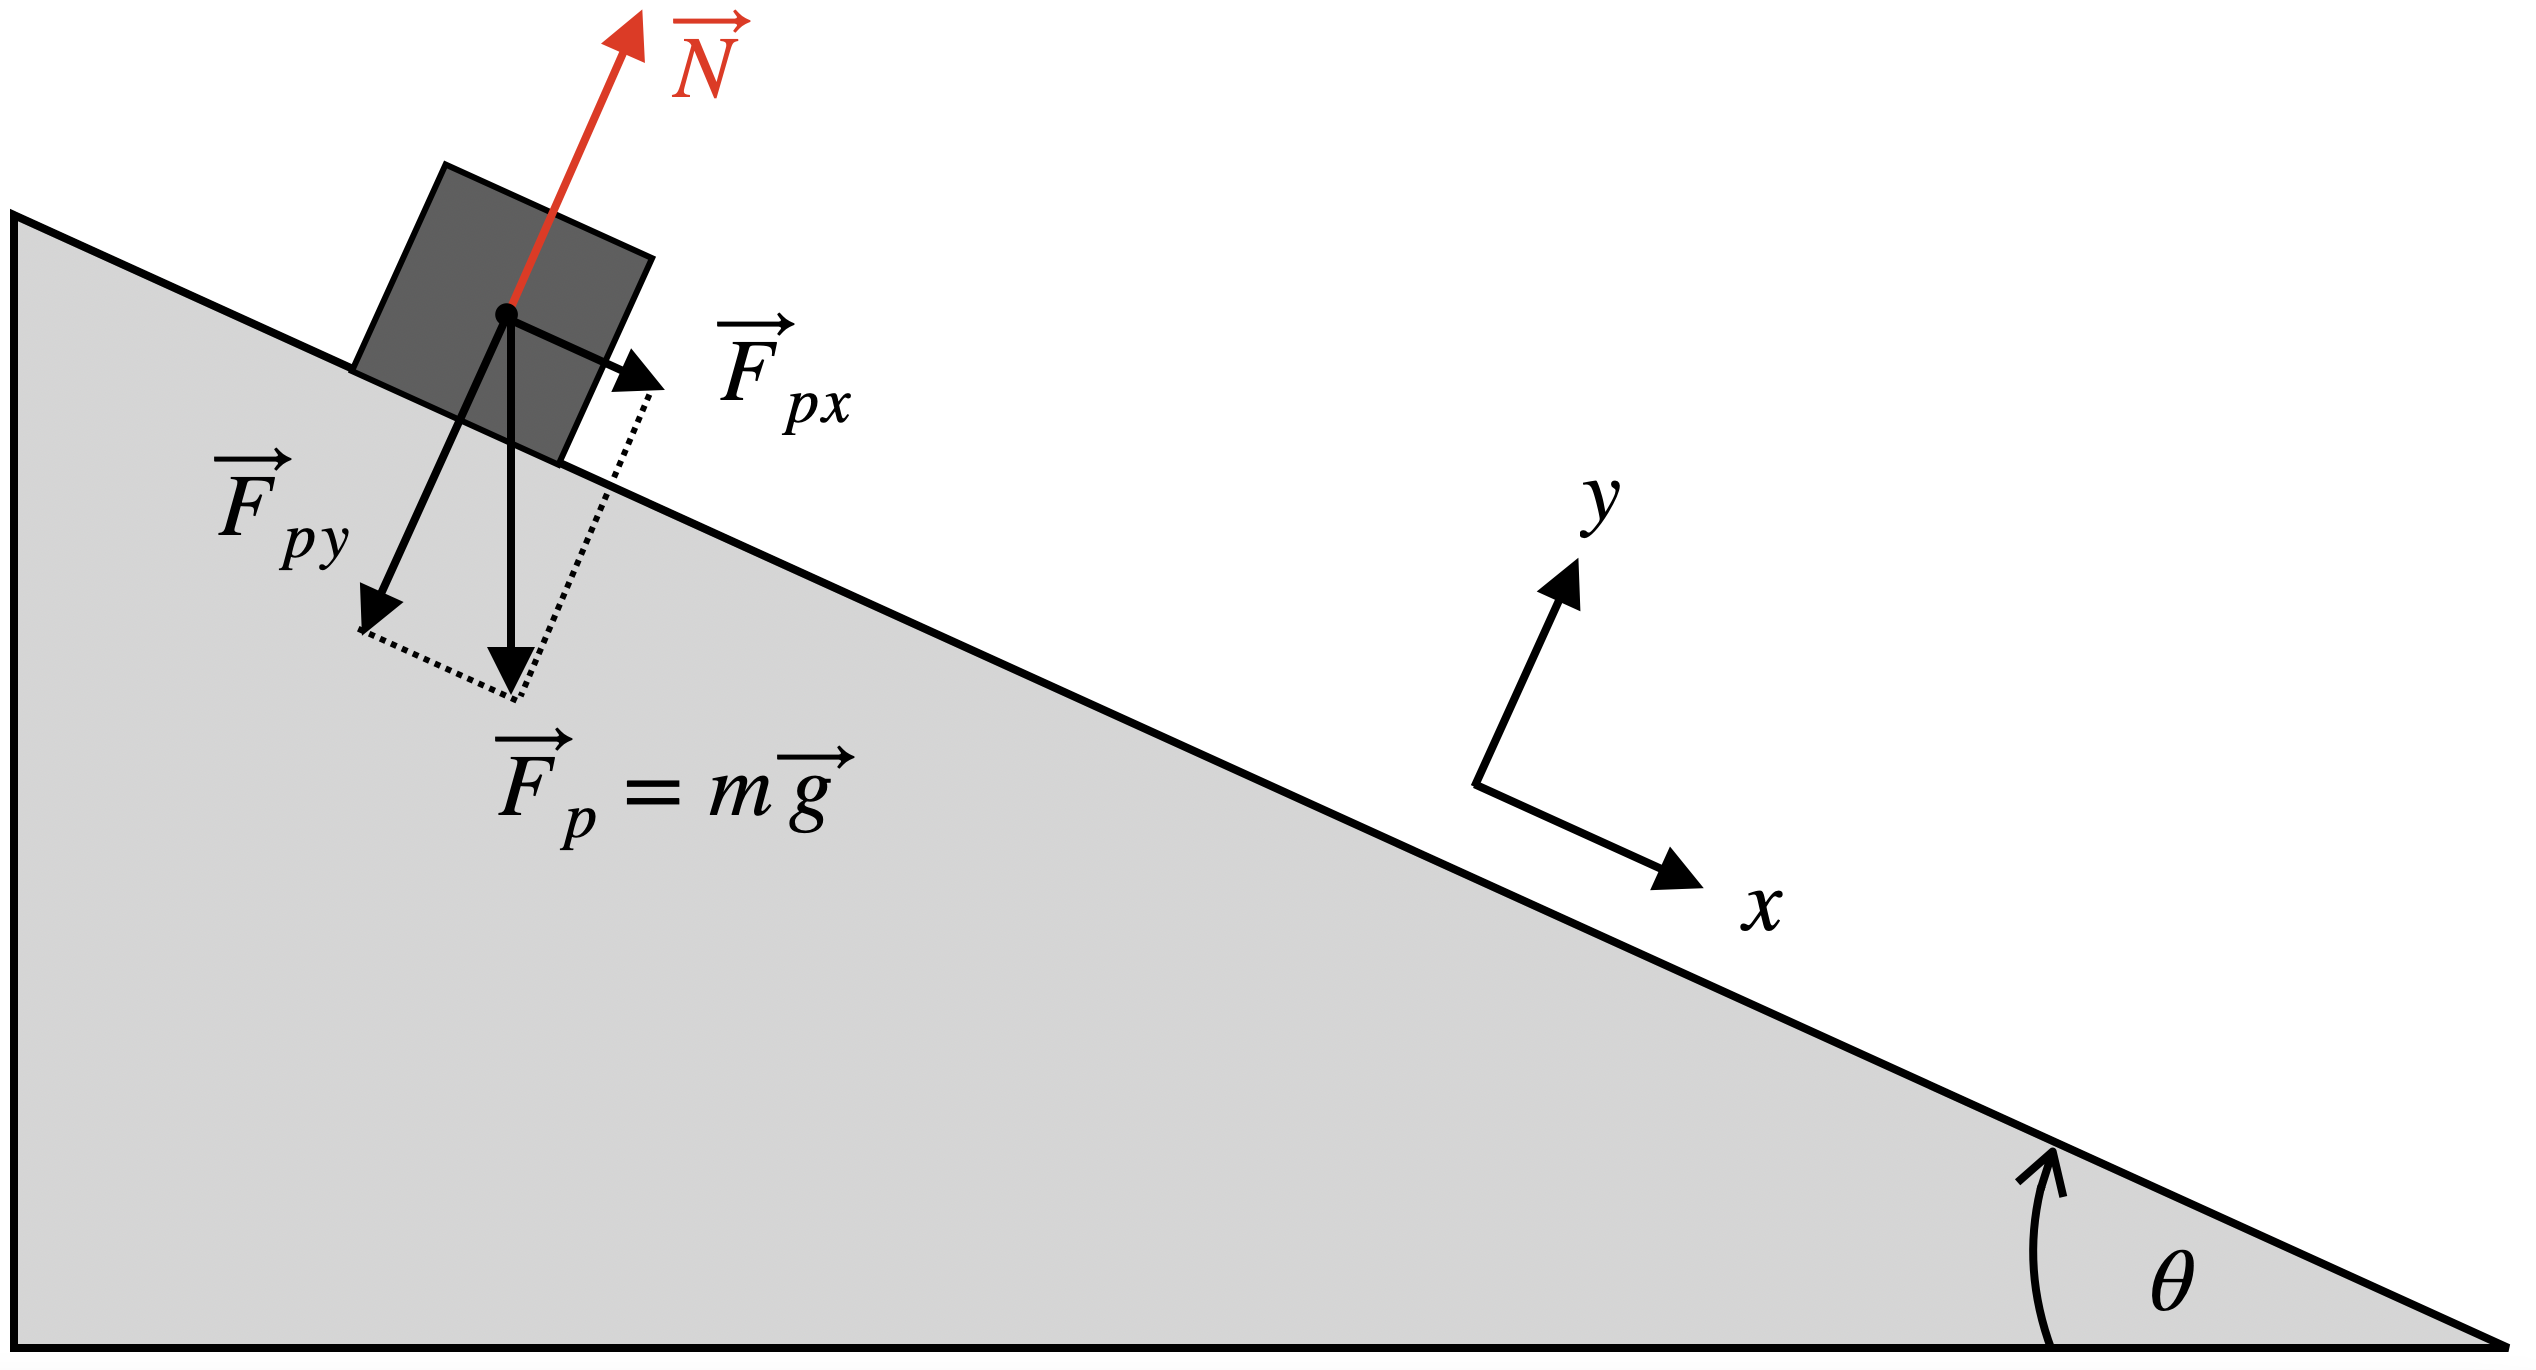
\includegraphics[width=10cm]{images/pianoincl.png}
        \caption{Rappresentazione di un piano inclinato con angolo $\theta$ e
        rappresentazione del sistema di riferimento scelto, con la coordinata $x$
        parallela al piano e la $y$ ortogonale.}
\end{center}
\label{fig:Iplain&pendulum:Iplain}
\end{figure}
\\
Nel caso con attrito avremo un moto solo se la componente parallela della
forza peso è maggiore della forza d'attrito massima:
\begin{equation}
    mg\sin\theta > \mu_s mg\cos\theta\seg \boxed{\tan\theta>\mu_s}
\end{equation}
Supponendo di trovarci in questa situazione, studiamo il caso dinamico:
\begin{equation}
    x:\quad mg\sin\theta -\mu_d mg\cos\theta = m\ddot x\seg
    \boxed{a_x = g\sx\sin\theta-\mu_d\cos\theta\dx}
\end{equation}
Dato che $\mu_d<\mu_s$, non può verificarsi il caso in cui $\tan\theta
=\mu_d$ che annullerebbe l'accelerazione lungo $x$.

\section{Pendolo semplice}
%---------------------------------------------------------------------------
\begin{figure}[htbp]
    \begin{center}
        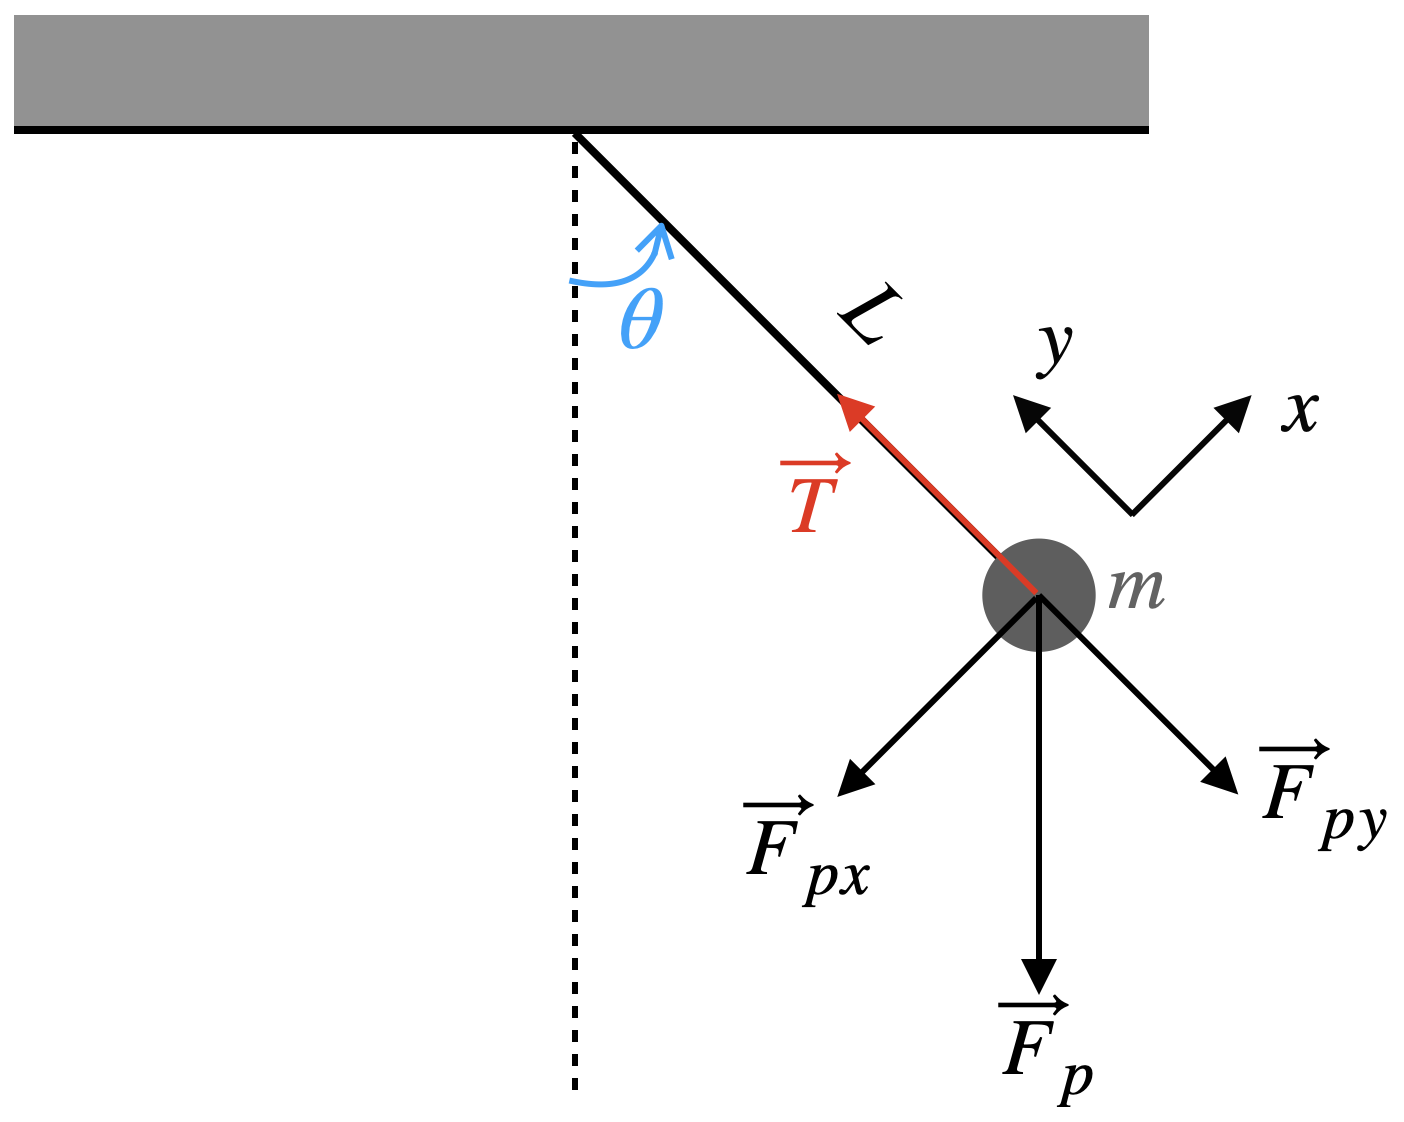
\includegraphics[width=10cm]{images/pendolo.png}
        \caption{Rappresentazione di un pendolo inclinato di un certo angolo
        $\theta$ rispetto alla verticale. È stato raffigurato anche il sistema
        di riferimento, con l'asse $y$ parallelo al filo di lunghezza $L$, e
        l'asse $x$ ortogonale ad esso.}
\end{center}
\label{fig:Iplain&pendulum:pendulum}
\end{figure}

Il pendolo è un sistema fisico costituito da un punto materiale di massa
$(m)$ sottoposto ad una forza costante, in questo caso la gravità, vincolato
ad avere una certa distanza $(L)$ da un punto fisso.\\
Nel caso mostrato in figura \ref{fig:Iplain&pendulum:pendulum}, la distanza
viene vincolata con un filo inestensibile teso con una tensione $(\vec T)$.
Vogliamo studiare la legge oraria dell'angolo $\theta$, l'angolo tra l'asse
verticale e la fune.\\
Scriviamo dunque le equazioni di Newton, considerando un asse parallelo alla
fune ed uno ortogonale.
\begin{equation}
    x:\quad -mg\sin\theta = ma_t\quad\quad y:\quad T-mg\cos\theta = ma_n
\end{equation}
\begin{equation}
    a_t = \frac{dv}{dt}=\frac d{dt}\sx L\dot\theta\dx=
    L\ddot\theta\quad\quad a_n = 0
\end{equation}
Lungo l'asse $y$ il corpo è in equilibrio, mentre lungo l'asse $x$ abbiamo
la seguente equazione differenziale:
\begin{equation}
    \boxed{\ddot\theta + \frac gL\sin\theta = 0}
\label{eq:pendulum_DE}
\end{equation}
Se consideriamo l'approssimazione di piccole oscillazioni, l'equazione differenziale appena ottenuta si riduce all'equazione dell'oscillatore armonico, in quanto:
\begin{equation}
    \theta \ll 1 \seg \sin\theta \sim \theta \seg
    \ddot\theta + \frac gL\theta = 0
\label{eq:pendulum_ODE}
\end{equation}
Dove la la pulsazione propria del sistema è $\omega_0 = \sqrt{\frac gL}$.
\begin{equation}
    \theta_{(t)} = \theta_0\sin\sx\omega_0t+\phi\dx\quad\quad
    \omega_{(t)} = \omega_0\theta_0\cos\sx\omega_0t+\phi\dx\quad\quad
    \theta_{(t)} =-\omega_0^2 \theta_0\sin\sx\omega_0t+\phi\dx
\end{equation}